This chapter describes the various ways and pieces the Kistl system is
programmed and customized.

\section{Objects}

\subsection{ObjectClass}

\subsection{Relation}
A \emph{Relation} defines the relationship between two Objects. Every Object can have zero or more \emph{Relations}.
\par
An example of a \emph{Relation} is the relation between \emph{Project} and \emph{Tasks}. One \emph{Project} can have zero or more \emph{Tasks}. One \emph{Tasks} must have a \emph{Project}.

\begin{figure}[ht]
	\begin{center}
		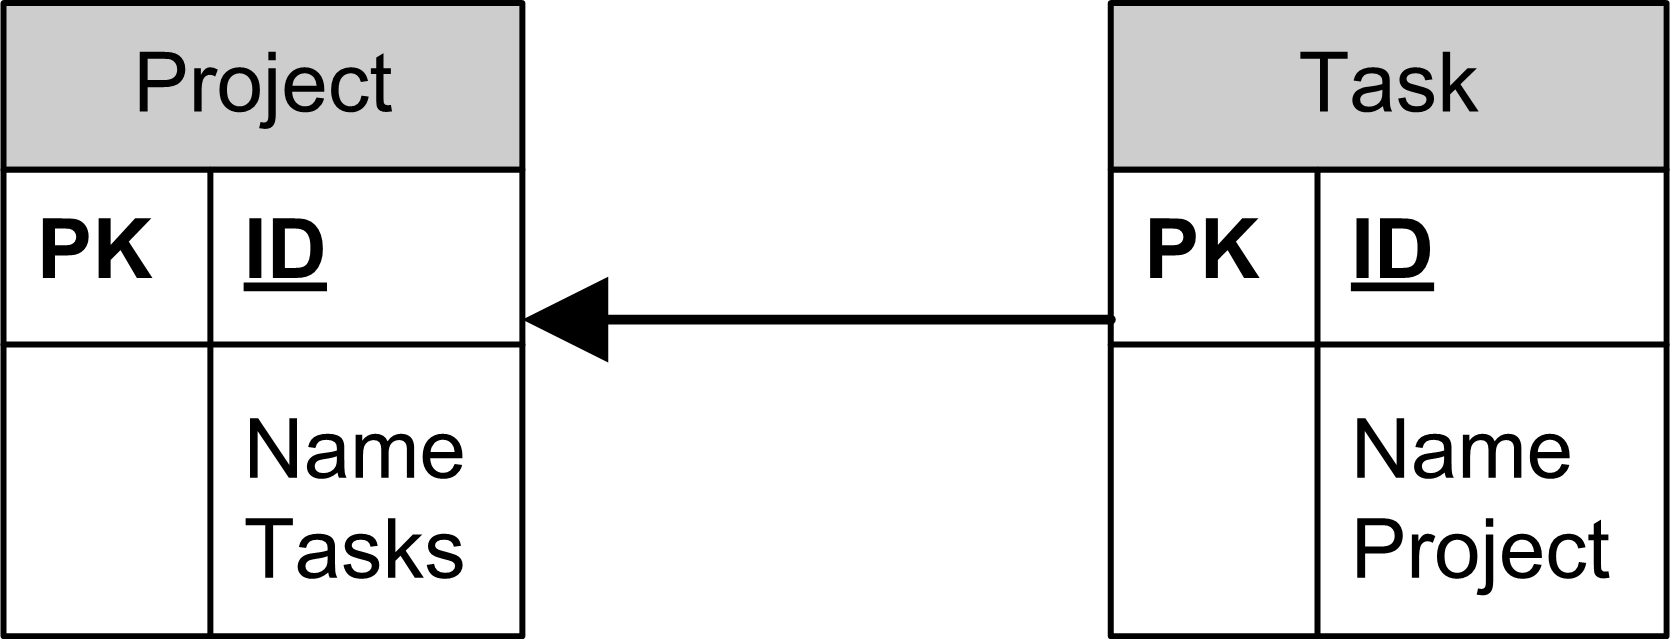
\includegraphics[width=0.6\textwidth]{images/Rel_1_n_Project_Tasks.png}
		\caption{Example for a \emph{Relation}}
		\label{example_for_relation}
	\end{center}
\end{figure}


% ----------------------------------------------------------------- Modeling relation -----------------------------------------------------------------
\subsubsection{Modeling a relation}
A Relation can be defined by creating an object of type \emph{Relation} and two \emph{RelationEnd} objects. This can be done by
\begin{itemize}
	\item creating an Relation Object. 
	\item invoking the \emph{Create Relation} method on an \emph{ObjectClass} instance.
\end{itemize}

\emph{RelationEnd} objects will be created automatically.

\par
Relations are edited in the \emph{Relation Editor}. The \emph{Relation Editor} is a custom \emph{FullObjectView} created by us.

\begin{figure}[ht]
	\begin{center}
		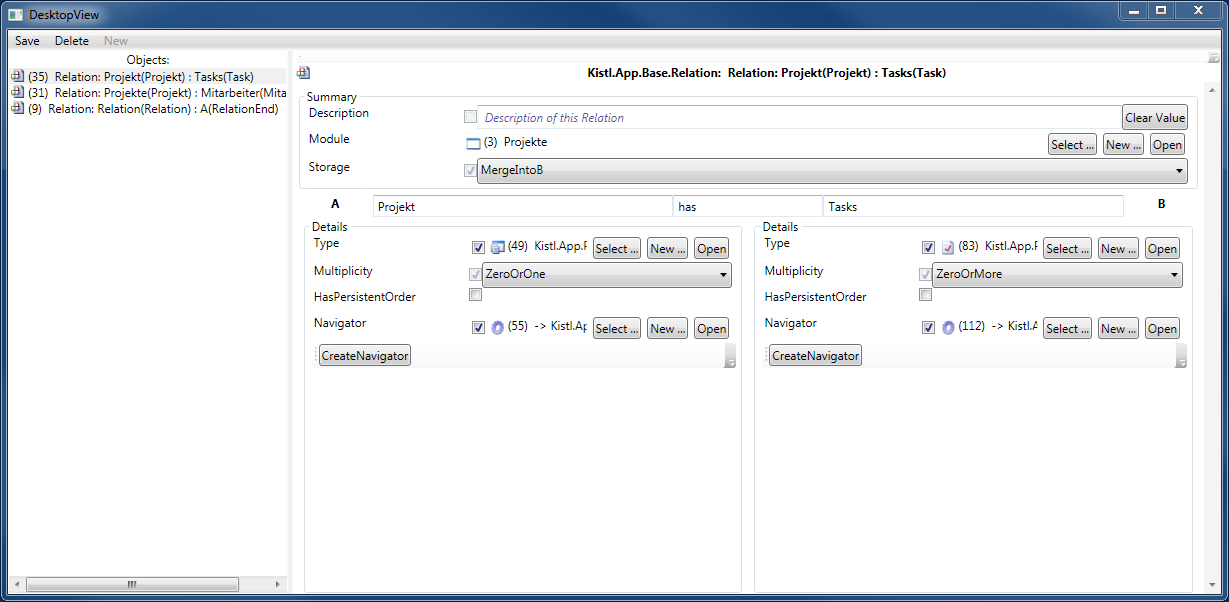
\includegraphics[width=0.9\textwidth]{images/ScreenShot_Rel_Project_Task.png}
		\caption{Example for editing a \emph{Relation}}
		\label{example_for_editing_relation}
	\end{center}
\end{figure}

% ----------------------------------------------------------------- Attributes of a relation -----------------------------------------------------------------
\subsubsection{Attributes of a relation}

\begin{figure}[ht]
	\begin{center}
		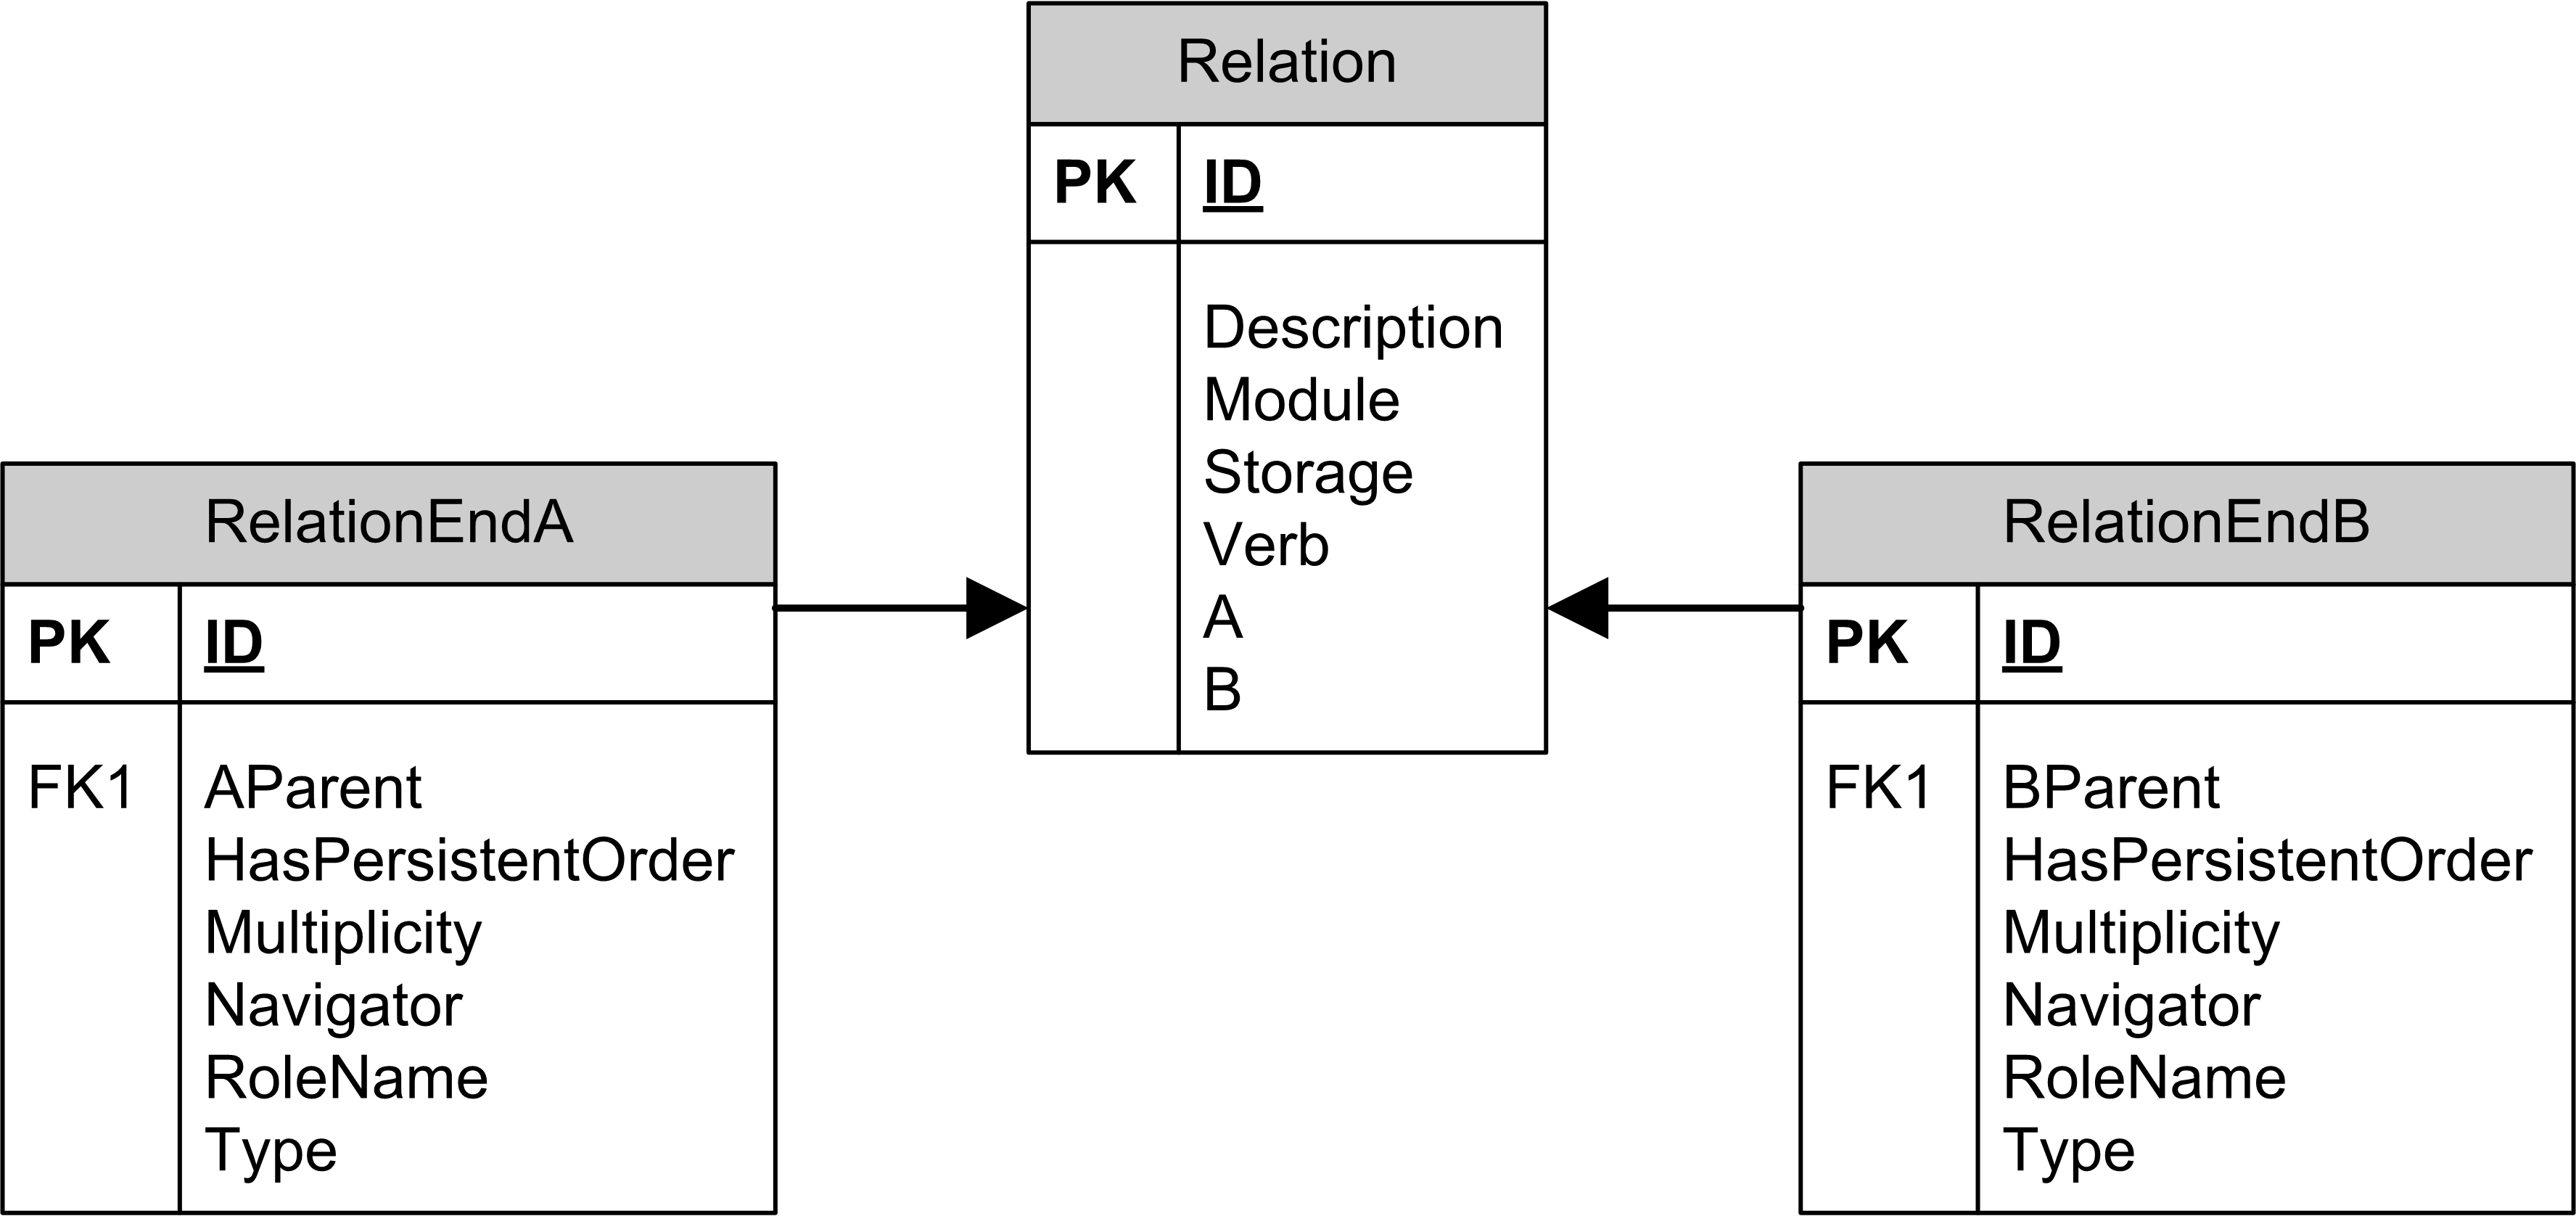
\includegraphics[width=0.9\textwidth]{images/Rel_Attributes.png}
		\caption{Attributes of a relation}
		\label{attributes_of_a_relation}
	\end{center}
\end{figure}

A \emph{Relation} has these attributes:
\begin{descriptionBorder}
	\item[Description] 	{ A text property used to describe the current relation }
	\item[Module] 		{ The \emph{Module} which is introducing the current relation }
	\item[Storage] 		{ The \emph{StorageType} of the current relation }
	\item[Verb] 		{ 	A verb used to name the current relation. 
							The verb is used in conjunction with the role names of the \emph{RelationEnd} objects to model a unique relation name. 
							This relation name will be used e.g. for the database FK Contraint name.}
	\item[A] 			{ The \emph{RelationEnd} A of the current relation }
	\item[B] 			{ The \emph{RelationEnd} B of the current relation }
\end{descriptionBorder}

A \emph{RelationEnd} has these attributes:
\begin{descriptionBorder}
	\item[AParent] { \emph{Relation} object if this \emph{RelationEnd} is the A-Side of the current relation. Otherwise \emph{NULL} }
	\item[BParent] { \emph{Relation} object if this \emph{RelationEnd} is the B-Side of the current relation. Otherwise \emph{NULL} }
	\item[HasPersistentOrder] { Specifies that the list is ordered. Applies only to lists  }
	\item[Multiplicity] { The \emph{Multiplicity} of the current \emph{RelationEnd} }
	\item[Navigator] { An optional \emph{Navigator} }
	\item[RoleName] { Name of the role of the current \emph{RelationEnd} }
	\item[Type] { \emph{ObjectClass} to which the current \emph{RelationEnd} points }
\end{descriptionBorder}

There are four \emph{StorageTypes} defined:
\begin{descriptionBorder}
	\item[MergeIntoA] { The relation information is stored with the A-side database table }
	\item[MergeIntoB] { The relation information is stored with the B-side database table }
	\item[Replicate] { The relation information is stored on both sides of the relations database tables }
	\item[Separate] { The relation information is stored in a separate database table }
\end{descriptionBorder}

There are three \emph{Multiplicities} defined:
\begin{descriptionBorder}
	\item[ZeroOrOne] { Optional Element (zero or one) }
	\item[One] { Required Element (exactly one) }
	\item[ZeroOrMore] { Optional List Element (zero or more) }
\end{descriptionBorder}

% ----------------------------------------------------------------- 1:n Relation -----------------------------------------------------------------
\subsubsection{1:n Relation}
A \emph{Project} can have zero or more \emph{Tasks}. A \emph{Task} may have one \emph{Project}.

\begin{figure}[ht]
	\begin{center}
		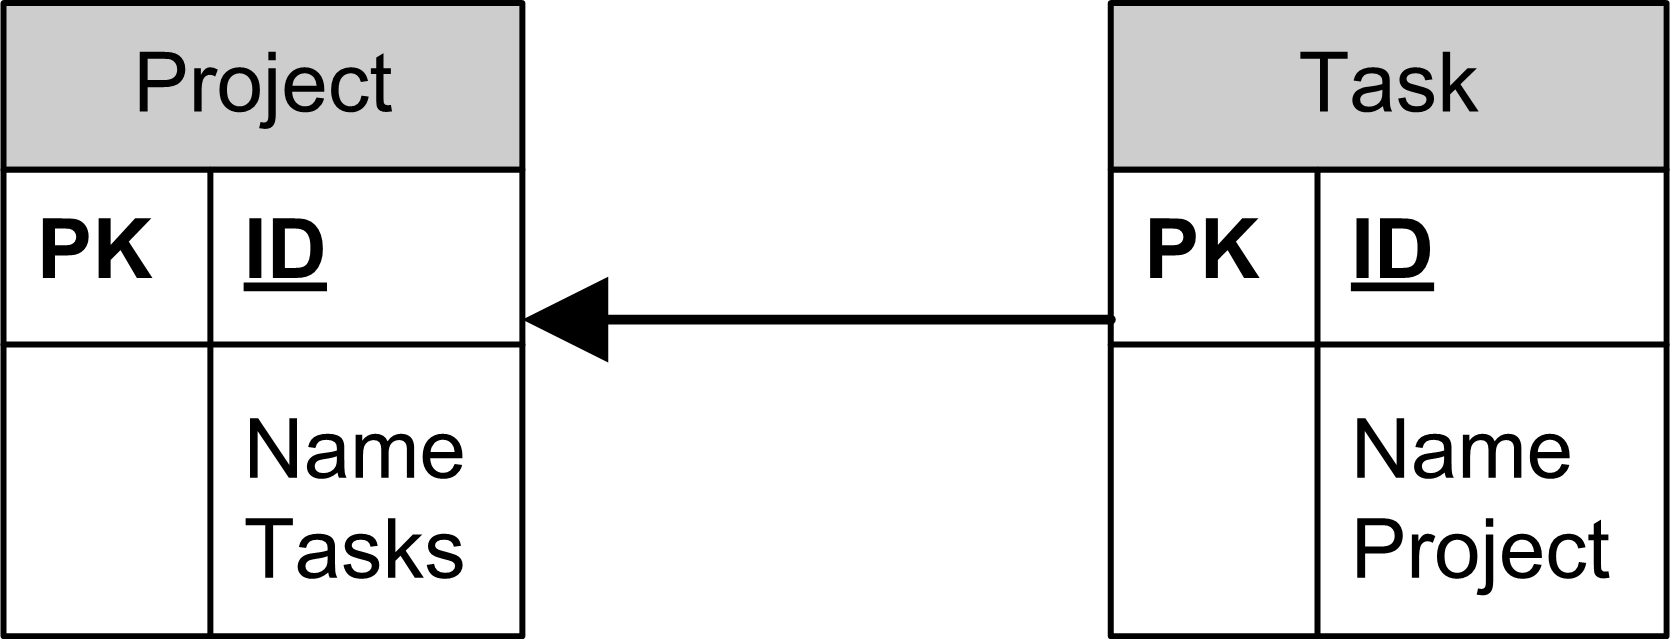
\includegraphics[width=0.6\textwidth]{images/Rel_1_n_Project_Tasks.png}
		\caption{Project/Tasks relation}
		\label{project_tasks_relation}
	\end{center}
\end{figure}

The \emph{Relation} object would be:
\begin{descriptionBorder}
	\item[Storage] 		{ = MergeIntoB }
	\item[Verb] 		{ = has }
\end{descriptionBorder}

The \emph{RelationEnd} A object would be:
\begin{descriptionBorder}
	\item[AParent] { = \emph{Relation}  }
	\item[BParent] { = \emph{NULL} }
	\item[HasPersistentOrder] { = false  }
	\item[Multiplicity] { = ZeroOrOne. If a \emph{Task} must have a \emph{Project} then One. }
	\item[Navigator] { = \emph{Navigator} to Tasks. The result would be a collection of \emph{Tasks} (ICollection\textless Task\textgreater) }
	\item[RoleName] { = Project }
	\item[Type] { = \emph{Task} instance of type \emph{ObjectClass} }
\end{descriptionBorder}

The \emph{RelationEnd} B object would be:
\begin{descriptionBorder}
	\item[AParent] { =  \emph{NULL} }
	\item[BParent] { = \emph{Relation} }
	\item[HasPersistentOrder] { = false  }
	\item[Multiplicity] { = ZeroOrMore }
	\item[Navigator] { = \emph{Navigator} to the parent \emph{Project}. The result would be a reference to a \emph{Project}  }
	\item[RoleName] { = Tasks }
	\item[Type] { = \emph{Project} instance of type \emph{ObjectClass} }
\end{descriptionBorder}

\begin{figure}[ht]
	\begin{center}
		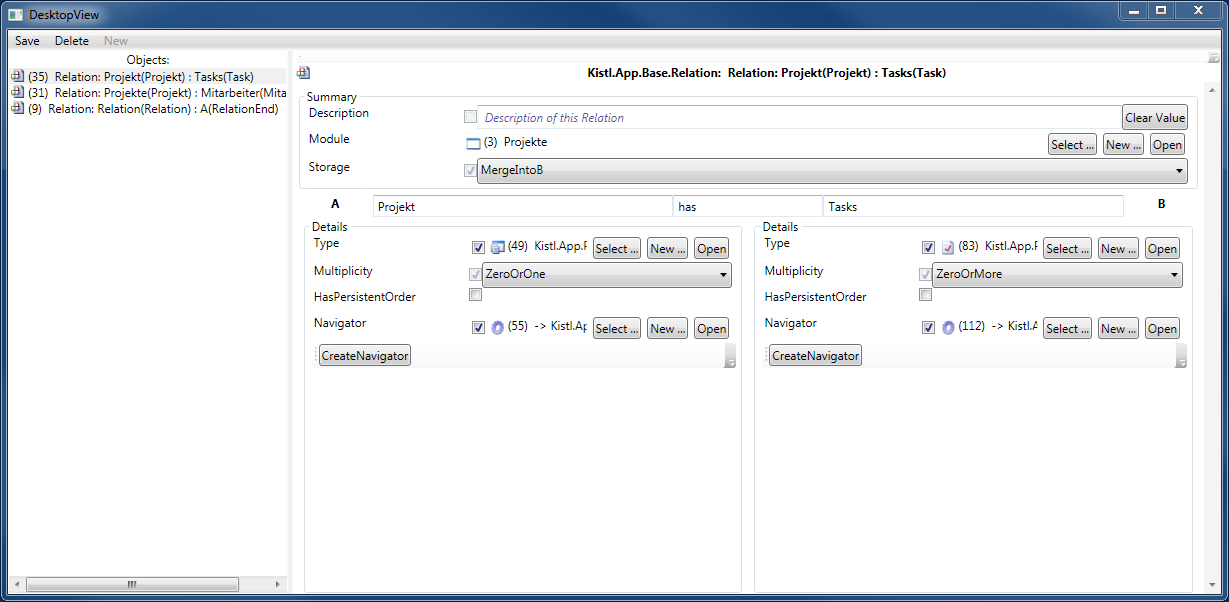
\includegraphics[width=0.9\textwidth]{images/ScreenShot_Rel_Project_Task.png}
		\caption{Editing the \emph{Project}/\emph{Tasks} relation}
		\label{editing_project_tasks_relation}
	\end{center}
\end{figure}

% ----------------------------------------------------------------- n:m Relation -----------------------------------------------------------------
\subsubsection{n:m Relation}
A \emph{Project} can have zero or more \emph{ProjectMembers}. A \emph{ProjectMember} can be assinged to zero or more \emph{Projects}.

\begin{figure}[ht]
	\begin{center}
		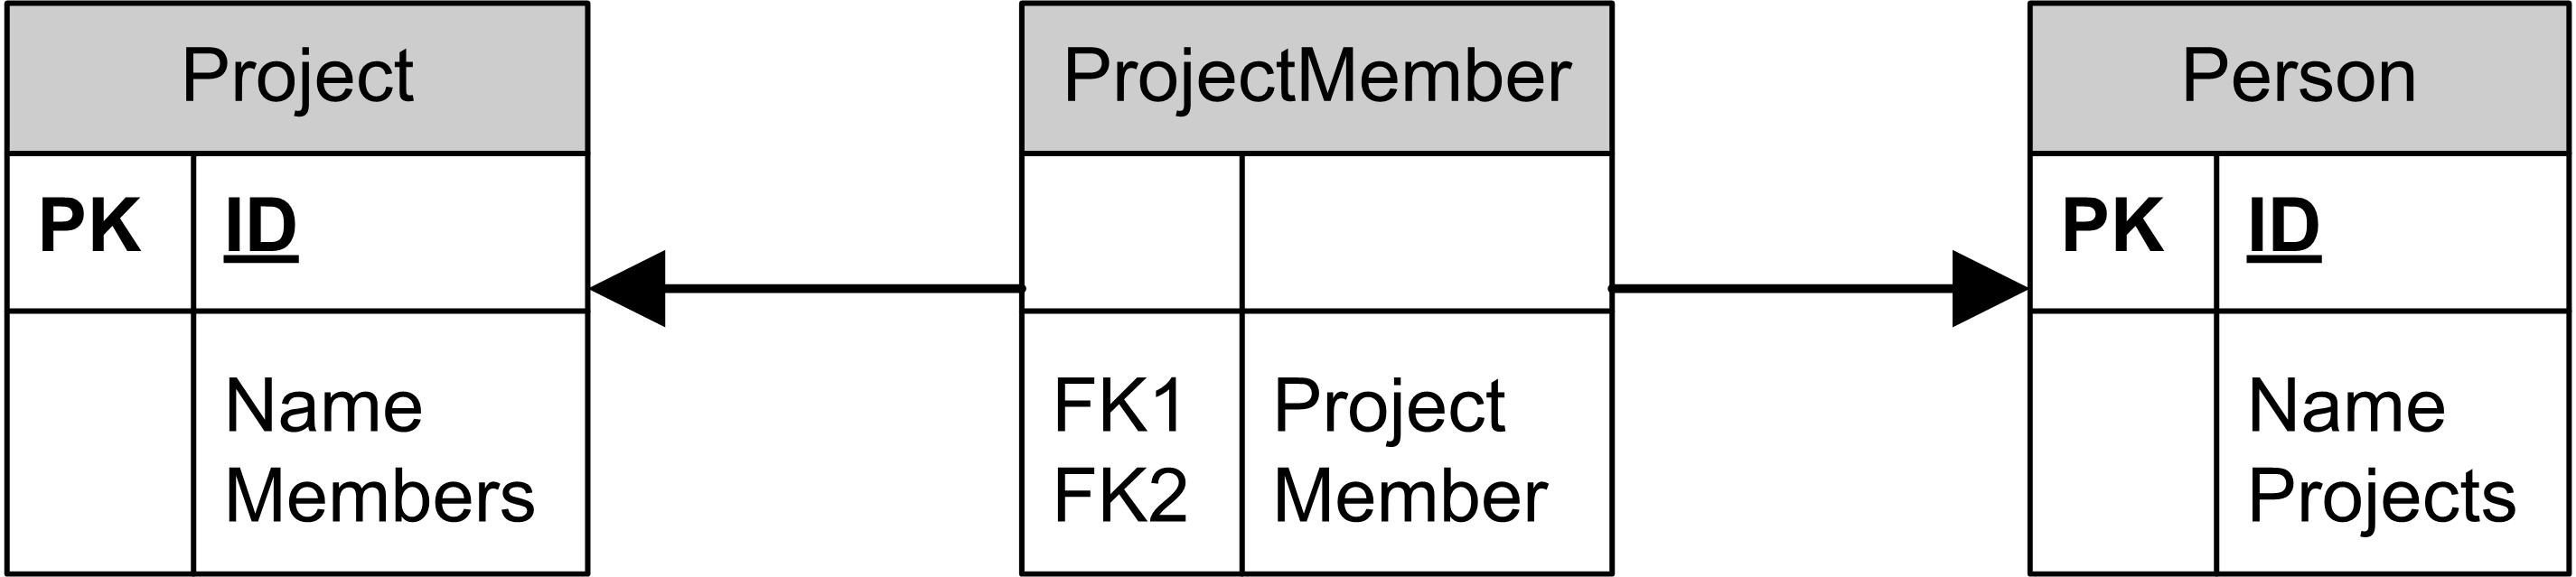
\includegraphics[width=0.6\textwidth]{images/Rel_n_m_Project_Member.png}
		\caption{Project/Member relation}
		\label{project_member_relation}
	\end{center}
\end{figure}

The \emph{Relation} object would be:
\begin{descriptionBorder}
	\item[Storage] 		{ = Seperate }
	\item[Verb] 		{ = has }
\end{descriptionBorder}

The \emph{RelationEnd} A object would be:
\begin{descriptionBorder}
	\item[AParent] { = \emph{Relation}  }
	\item[BParent] { = \emph{NULL} }
	\item[HasPersistentOrder] { = true  }
	\item[Multiplicity] { = ZeroOrMore. }
	\item[Navigator] { = \emph{Navigator} to Persons. The result would be a list of \emph{Persons} (IList\textless Person\textgreater) }
	\item[RoleName] { = Projects }
	\item[Type] { = \emph{Person} instance of type \emph{ObjectClass} }
\end{descriptionBorder}

The \emph{RelationEnd} B object would be:
\begin{descriptionBorder}
	\item[AParent] { =  \emph{NULL} }
	\item[BParent] { = \emph{Relation} }
	\item[HasPersistentOrder] { = true  }
	\item[Multiplicity] { = ZeroOrMore }
	\item[Navigator] { = \emph{Navigator} to the assigned \emph{Projects}. The result would be a list of \emph{Projects} (IList\textless Project\textgreater)  }
	\item[RoleName] { = Member }
	\item[Type] { = \emph{Project} instance of type \emph{ObjectClass} }
\end{descriptionBorder}

\begin{figure}[ht]
	\begin{center}
		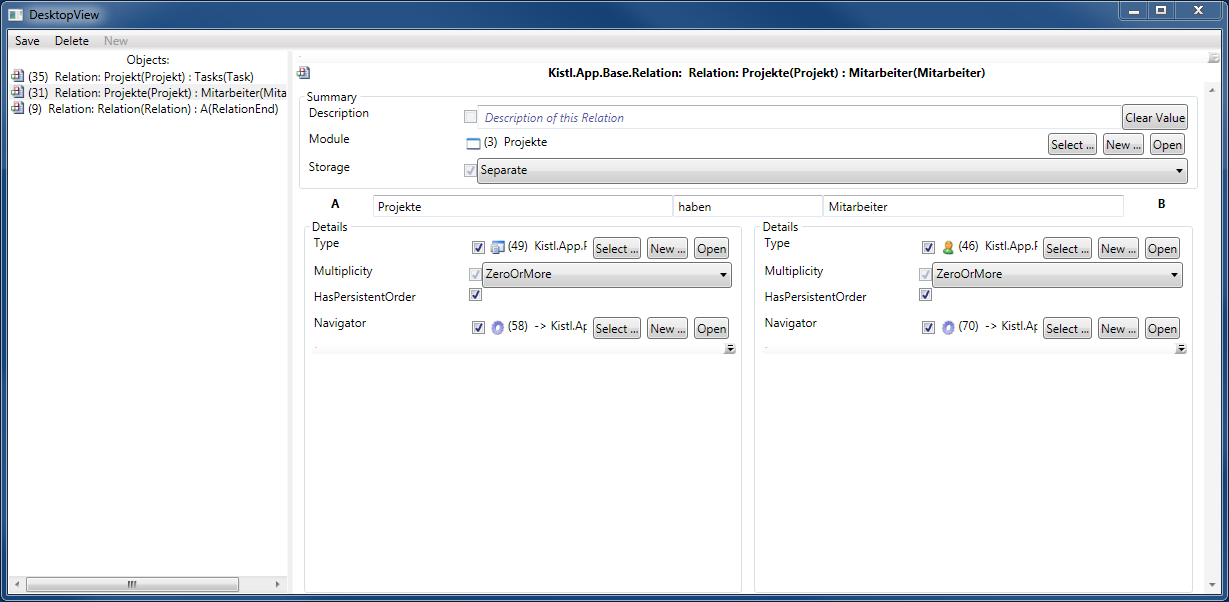
\includegraphics[width=0.9\textwidth]{images/ScreenShot_Rel_Project_ProjectMember.png}
		\caption{Editing the \emph{Project}/\emph{Member} relation}
		\label{editing_project_member_relation}
	\end{center}
\end{figure}

% ----------------------------------------------------------------- 1:1 Relation -----------------------------------------------------------------
\subsubsection{1:1 Relation}
A \emph{Relation} must have a \emph{RelationEnd} A. A \emph{RelationEnd} may have a AParent \emph{Relation} if it's a A \emph{ReleationEnd}.

\begin{figure}[ht]
	\begin{center}
		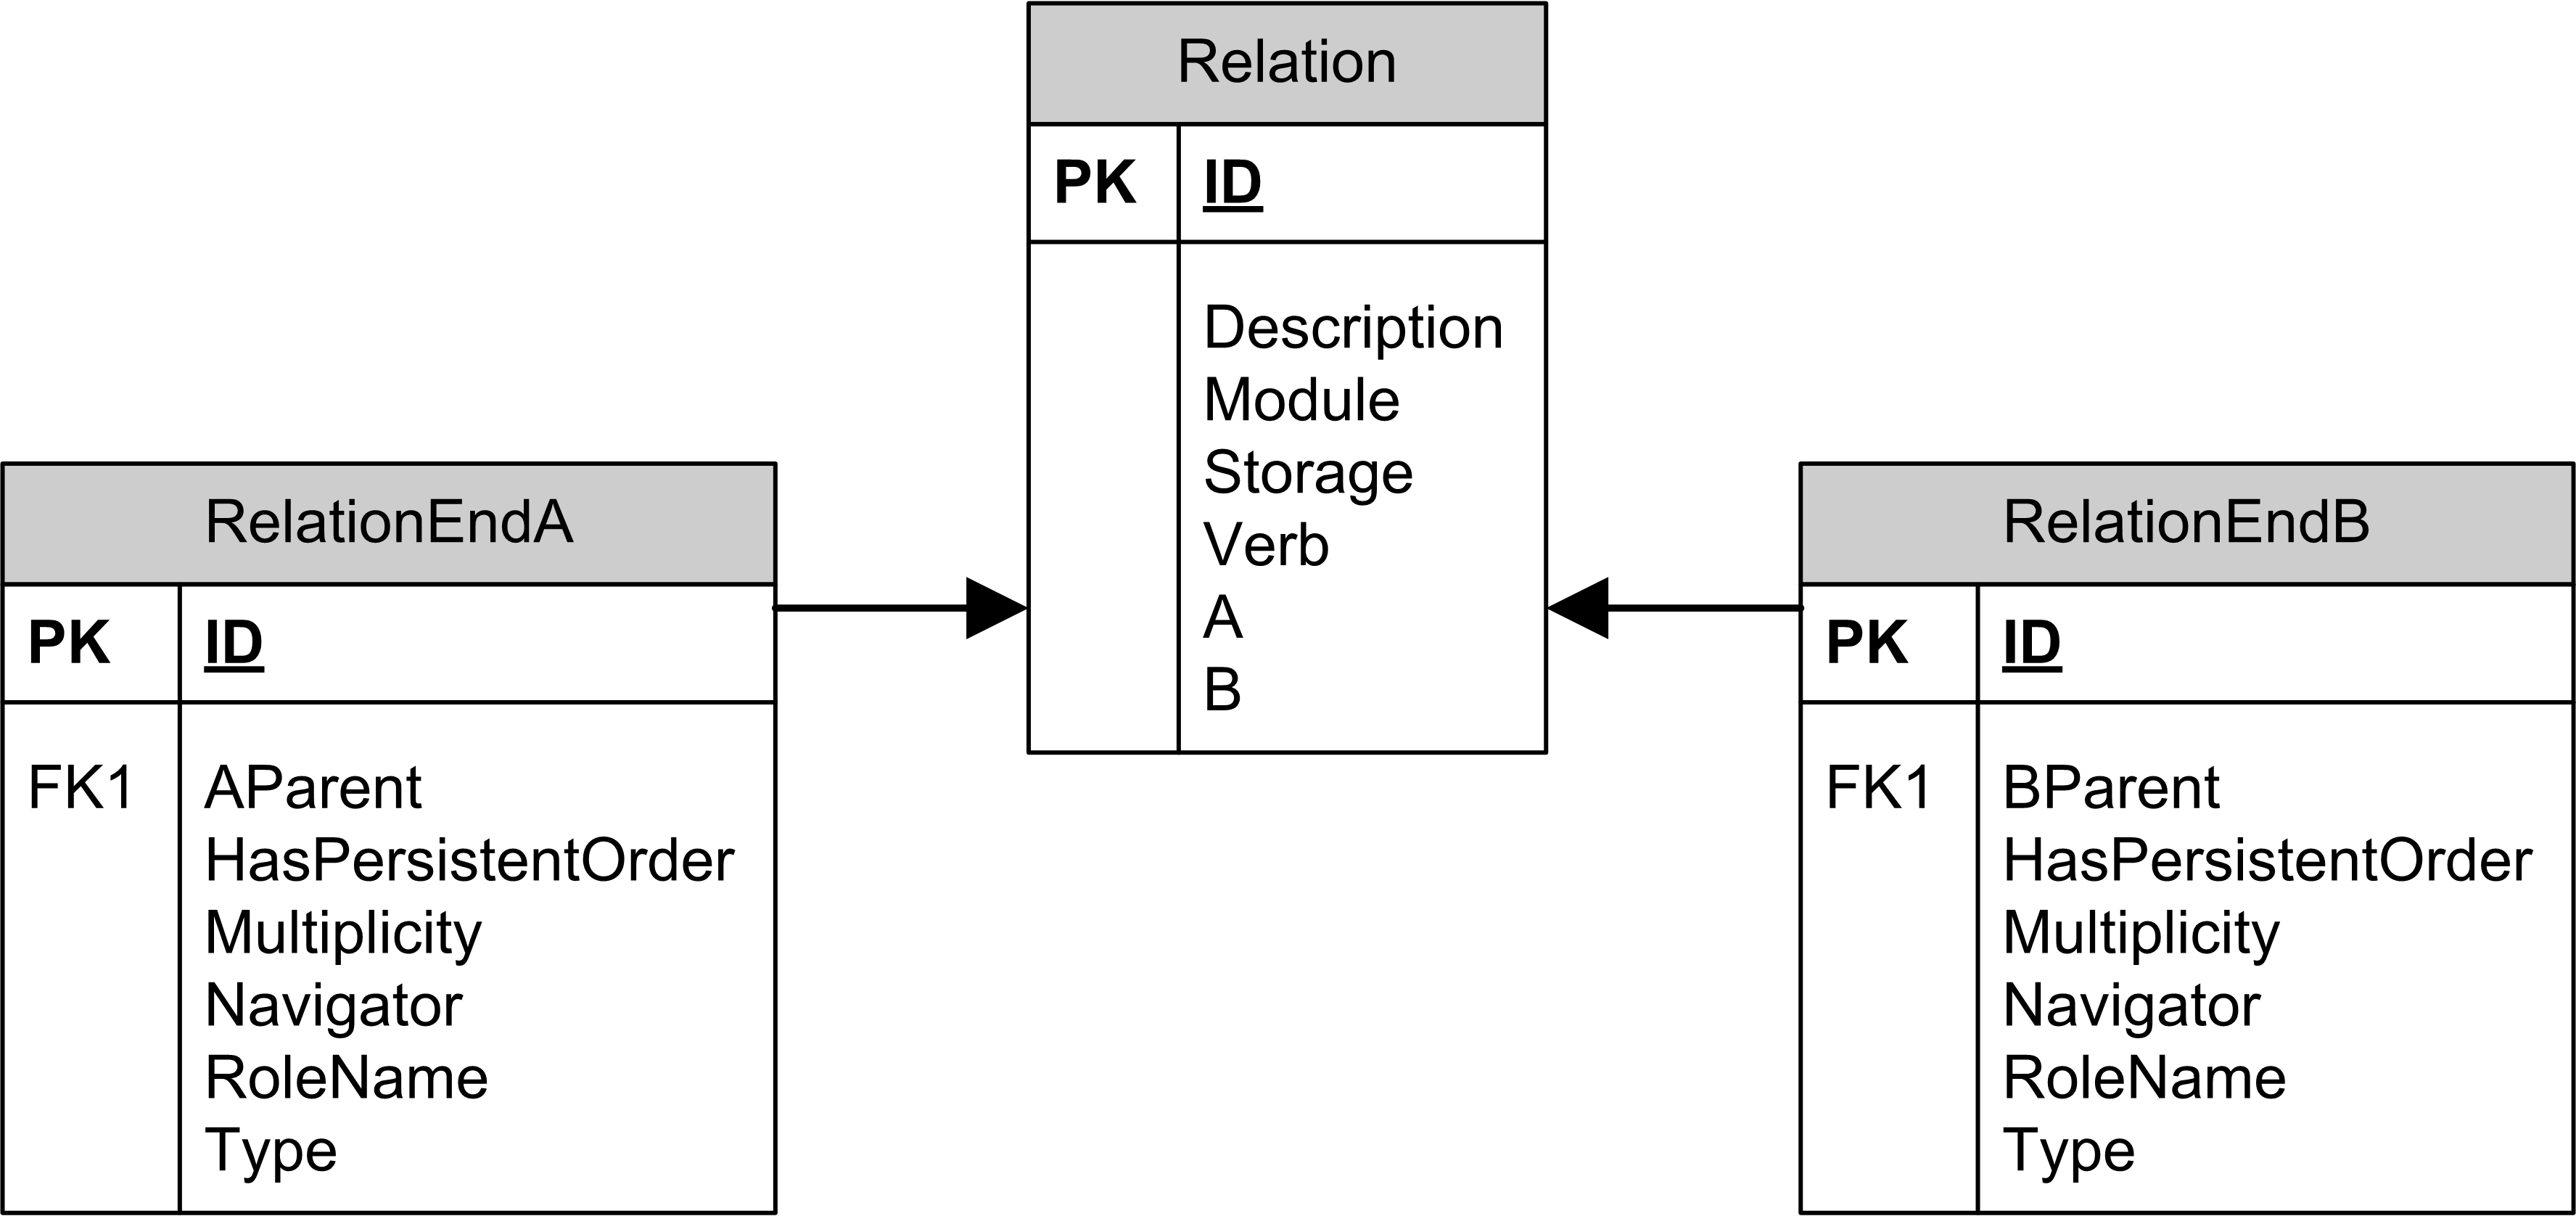
\includegraphics[width=0.9\textwidth]{images/Rel_Attributes.png}
		\caption{Relation/RelationEnd relation}
		\label{relation_relationend_relation}
	\end{center}
\end{figure}

The \emph{Relation} object would be:
\begin{descriptionBorder}
	\item[Storage] 		{ = MergeIntoA }
	\item[Verb] 		{ = hasA }
\end{descriptionBorder}

The \emph{RelationEnd} A object would be:
\begin{descriptionBorder}
	\item[AParent] { = \emph{Relation}  }
	\item[BParent] { = \emph{NULL} }
	\item[HasPersistentOrder] { = false  }
	\item[Multiplicity] { = ZeroOrOne }
	\item[Navigator] { = \emph{Navigator} to \emph{RelationEnd}. The result would be a reference to a \emph{RelationEnd} }
	\item[RoleName] { = Relation }
	\item[Type] { = \emph{RelationEnd} instance of type \emph{ObjectClass} }
\end{descriptionBorder}

The \emph{RelationEnd} B object would be:
\begin{descriptionBorder}
	\item[AParent] { =  \emph{NULL} }
	\item[BParent] { = \emph{Relation} }
	\item[HasPersistentOrder] { = true  }
	\item[Multiplicity] { = One }
	\item[Navigator] { = \emph{Navigator} to the assigned \emph{Relation}. The result would be a reference to a \emph{Relation}  }
	\item[RoleName] { = A }
	\item[Type] { = \emph{Relation} instance of type \emph{ObjectClass} }
\end{descriptionBorder}

\begin{figure}[ht]
	\begin{center}
		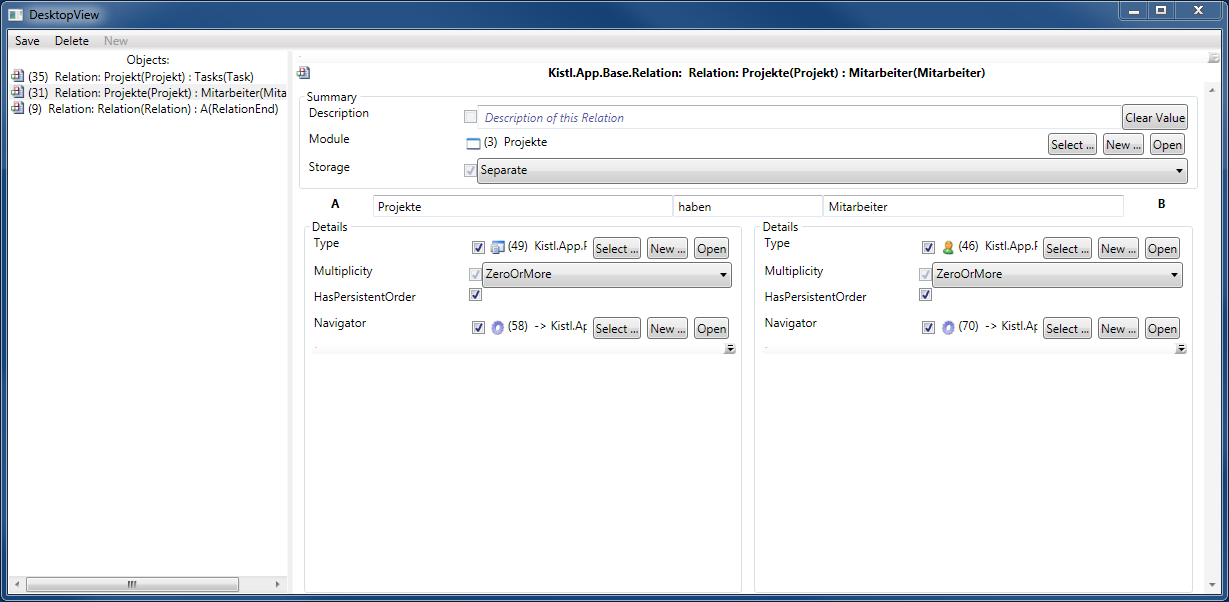
\includegraphics[width=0.9\textwidth]{images/ScreenShot_Rel_Project_ProjectMember.png}
		\caption{Editing the \emph{Relation}/\emph{RelationEnd} relation}
		\label{editing_relation_relationend_relation}
	\end{center}
\end{figure}

% ----------------------------------------------------------------- Multiplicity summary -----------------------------------------------------------------
\subsubsection{Multiplicity and StorageType summary}

\begin{center}
	\begin{tabular}{|p{5cm}|p{5cm}|}
	\hline
		\multicolumn{2}{|c|}{\textbf{1:n}} \\ 
		\multicolumn{2}{|c|}{ Storage = MergeIntoB } \\
	\hline
		\multicolumn{1}{|c|}{\textbf{A}} & \multicolumn{1}{|c|}{\textbf{B}} \\
	\hline
		A.Nav is a collection & B.Nav is nullable \\
		Multiplicity = ZeroOrOne & Multiplicity = ZeroOrMore \\
	\hline
		A.Nav is a collection & B.Nav is not nullable\\
		Multiplicity = One  & Multiplicity = ZeroOrMore \\
	\hline
	\end{tabular}
\end{center}

\begin{center}
	\begin{tabular}{|p{5cm}|p{5cm}|}
	\hline
		\multicolumn{2}{|c|}{\textbf{n:1}} \\ 
		\multicolumn{2}{|c|}{ Storage = MergeIntoA } \\
	\hline
		\multicolumn{1}{|c|}{\textbf{A}} & \multicolumn{1}{|c|}{\textbf{B}} \\
	\hline
		A.Nav is nullable & B.Nav is a collection \\
		Multiplicity = ZeroOrMore & Multiplicity = ZeroOrOne\\
	\hline
		A.Nav is not nullable & B.Nav is a collection \\
		Multiplicity = ZeroOrMore & Multiplicity = One \\
	\hline
	\end{tabular}
\end{center}

\begin{center}
	\begin{tabular}{|p{5cm}|p{5cm}|}
	\hline
		\multicolumn{2}{|c|}{\textbf{n:m}} \\ 
		\multicolumn{2}{|c|}{ Storage = Seperate } \\
	\hline
		\multicolumn{1}{|c|}{\textbf{A}} & \multicolumn{1}{|c|}{\textbf{B}} \\
	\hline
		A.Nav is a collection & B.Nav is a collection \\
		Multiplicity = ZeroOrMore & Multiplicity = ZeroOrMore \\
	\hline
	\end{tabular}
\end{center}

\begin{center}
	\begin{tabular}{|p{5cm}|p{5cm}|}
	\hline
		\multicolumn{2}{|c|}{\textbf{1:1}} \\ 
		\multicolumn{2}{|c|}{ Storage = MergeIntoA } \\
		\multicolumn{2}{|c|}{ Storage = MergeIntoB } \\
		\multicolumn{2}{|c|}{ Storage = Replicate (Not supported yet) } \\
	\hline
		\multicolumn{1}{|c|}{\textbf{A}} & \multicolumn{1}{|c|}{\textbf{B}} \\
	\hline
		A.Nav is nullable & B.Nav is nullable \\
		Multiplicity = ZeroOrOne & Multiplicity = ZeroOrOne \\
	\hline
		A.Nav is nullable & B.Nav is not nullable \\
		Multiplicity = One & Multiplicity = ZeroOrOne \\
	\hline
		A.Nav is not nullable & B.Nav is nullable \\
		Multiplicity = ZeroOrOne & Multiplicity = One \\
	\hline
		A.Nav is not nullable & B.Nav is not nullable \\
		Multiplicity = One & Multiplicity = One \\
	\hline
	\end{tabular}
\end{center}



\subsection{Additional Metadata}

The object model is intended to be very rich and provide the various
subsystems with meta data directly from the \emph{ObjectClass}.

This section describes the various pieces of this meta data.

\subsubsection{New related objects}

A \emph{CreateRelatedUseCase} describes the use case of creating a new
object related to the "current" instance. One such use case would be
e.\,g.~"create a new \emph{Relation} from the current ObjectClass."

Such use cases are described with \emph{CreateRelatedUseCase} objects:

\begin{CS}
interface CreateRelatedUseCase
{
	string Label;
	Method Action;
	Relation AffectedRelation; // optional
}
\end{CS}

The \emph{Action} will be called when the user requests an execution of
this use case. This method doesn't take any parameters and returns the
newly created object. The infrastructure on the client will cause the
returned object to be displayed to the user. The business logic should
already have filled out the property values according to the use case.
The name of the method should start with "Create".

If the optional \emph{AffectedRelation} is specified, one of its ends it
must match the \emph{ObjectClass} of the \emph{Method}. This relation
can then be used to identify controls in the UI where the action can be
placed.

\section{Modules}

\section{Compound Objects}
Lets say there is a \emph{PhoneNumber} Compound Object.
\begin{CS}
class PhoneNumber
{
	string CountryCode;
	string AreaCode;
	string Number;
	string Extension;
}
\end{CS}

A Person has two phone numbers:

\begin{CS}
class Person
{
	string Name;
	...
	PhoneNumber  Tel;
	PhoneNumber? Fax;
}
\end{CS}
\emph{Tel} is not nullabe, \emph{Fax} is nullable.

\subsection{Accessing Compound Objects}

\begin{itemize}
	\item{If a compound object property is not nullable then the content of the property is always a valid reference.}
	\item{If a compound object property is  nullable then the content of the property may be null.}
\end{itemize}

\begin{CS}
Person p;
string number;

number = p.Tel.Number;
number = p.Fax.Number; // throws NullReferenceException if Fax is null

p.Tel.Number = "12345678";
p.Fax.Number = "12345678"; // throws NullReferenceException if Fax is null

PhoneNumber n;

n = p.Tel; // returnes a reference of the compound object
n.Number = "87654321"; // changes p.Tel.Number
n = p.Fax; // may be null
n.Number = "87654321"; // changes p.Fax.Number or throws NullReferenceException if Fax is null

p.Fax = p.Tel; // sets p.Fax equals to p.Tel - same reference
p.Fax = (PhoneNumber)p.Tel.Clone(); // sets p.Fax to a copy of p.Tel
p.Fax.Number = "87654321"; // changes p.Fax.Number but does not change p.Tel.Number

p.Tel = null; // throws a ArgumentNullException
p.Fax = null; // sets Fax to null

n = ctx.CreateStruct<PhoneNumber>(); // creates a new PhoneNumber Struct;
n.Number = "12345678";
p.Tel = n; // sets p.Tel to n
p.Tel.Number = "18273645"; // changes p.Tel.Number and n.Number
n.Number = "87654321"; // changes n.Number and p.Tel.Number
\end{CS}

\section{Enhancing Kistl's inner workings}

\subsection{Database Providers}

\section{Graphical User Interface}

Like other subsystems, the GUI core is designed to be platform
independent. Therefore only the "outermost" shell contains toolkit
specific code.

\subsection{Architecture}

The GUI is modeled after the Model-View-ViewModel architecture. The
\emph{Model} represents the underlying data structures and business
logic. It is provided by the generated classes from the actual
datamodel. \emph{View Models} or \emph{presentable} models provide
display specific functionality like formatting, transient state holding
and implementing the user's possible actions. They always inherit from
\emph{Kistl.Client.Presentables.PresentableModel}.
Common implementations reside in the
\emph{Kistl.Client.Presentables} namespace. Finally,
\emph{Views} (editors and displays) are the actual components taking
care of showing content to the user and converting the users keypresses
and clicks into calls on the view models interface.  Views are
toolkit\footnote{Toolkits are GUI libraries like WPF, GTK\# or Windows
Forms but can also be implemented by more complex providers such as
ASP.NET.} specific and reside in the toolkit's respective assembly.

This architecture decouples the actual functionality of the Model and
the View Model completly from the inner workings of a toolkit and
thereby maximise the reuse of code between different clients.

\subsection{Plumbing}

The three layers are connected through two sets of descriptors. The
\emph{PresentableModelDescriptor}s contain information about the
available View Models and their preferred way of being displayed. The
\emph{ViewDescriptor}s link \emph{PresentableModelDescriptor}s with
the controls capable of displaying them.

\subsubsection{Presentable Model Descriptors}

Currently there exist three major types of View Models. 

\begin{description}

\item[\emph{DataObjectModel}s]{represent a complete data object;
provide standardised access to properties; provide non-standard Views
with additional functionality; selected via
\emph{ObjectClass.DefaultPresentableModelDescriptor}}

\item[\emph{ValueModel}s]{represent a specific piece of data;
representations of Properties are selected via
\emph{Property.ValueModelDescriptor}; method results are currently
created directly via \emph{Factory.CreateSpecificModel}}

\item[other Presentables]{represent objects in the View which do not
have persistent representations, like dialogs or wizards; always
created by calling \emph{Factory.CreateSpecificModel}}

\end{description} 

\subsubsection{View Descriptors}

These descriptors list the available Views by Toolkit and which subset
of Presentables they are able to work with.

\subsubsection{Control Kind}

The \emph{ControlKind} specifies the toolkit-independent kind or type of
control that should display a given Presentable. While the View
specifies the Control Kind it implements the Presentable requests a
specific Kind to be displayed via the
\emph{PresentableModelDescriptor.DefaultControlKind} value.

In special situations this default value can be overridden. For example,
the metadata of a property contains a \emph{RequestedControlKind} which
is used instead of the \emph{DefaultControlKind} when present. If there
is no View matching the requested Kind, the infrastructure may either
fall back to the default control kind, or use a similar control kind
from higher up in the hierarchy.

Typical kinds of controls:

\begin{description}

\item[WorkspaceWindow] {the top-level control within which all user
interaction happens}

\item[SelectionTaskDialog] {a dialog letting the user select something
from a longer list of items}

\item[ObjectView] {display the modeled object in full}

\item[ObjectListEntry] {display the modeled object as item in a list}

\item[TextEntry] {lets the user edit a property as text}

\item[IntegerSlider] {lets the user edit a number with a slider}

\item[YesNoCheckbox] {a simple yes/no checkbox}

\item[YesNoOtherText] {radio buttons allowing one to select either "yes",
"no" or a TextEntry field}

\item[ExtendedYesNoCheckbox] {a checkbox with additional text as label}

\end{description}

The kind of a control is identified by the \emph{ControlKind}'s class. The
hierarchy between different kinds of controls is modeled with inheritance.

Control Kinds can also be used to configure the actual control. This
possibility should be used sparingly as a control should instead seek to
infer its configuration from the underlying Presentable. For example, an
integer slider control should lookup the minimal and maximal allowed
values in the underlying \emph{IntegerRangeConstraint} while an
ExtendedYesNoCheckbox has no other place to retrieve the new label.

\subsection{Asynchronous Loading}

\emph{Not yet implemented.}

To facilitate low-latency user interfaces, the ViewModels should implement a
thin proxy layer to delegate all potential blocking operations onto a worker
thread. To keep programming this layer easy, there are a few helper classes and
a few constraints on the available interface mechanisms as well as a consistent
contract over all compliant ViewModels.

There are only three ways to communicate over the \emph{thread gap}:
\begin{enumerate}
\item{accessing a property}
\item{calling a \emph{void} function (with not \emph{out} or \emph{ref} parameters)}
\item{having an \emph{EventHandler} called}
\end{enumerate}

All compliant ViewModels provide a \emph{IsLoading} property that signifies
whether any background processing is active. While this property is true, any
value read from a property may be stale and/or about to be replaced. Changes to
the visible value of a property are always reported via the
\emph{PropertyChanged} event from the \emph{INotifyPropertyChanged} interface.
This should suffice for enabling binding frameworks to show current values to
the user: When reading a value from a property, a cached value is returned
immediately and optionally a refresh is triggered, which in turn may cause a
PropertyChanged event a little bit later.

In the case of time-dependent values, the ViewModel has to take care
to establish a periodic refresh timer\footnote{Todo: such a timer should be
provided by the infrastructure for platform dependent refreshing} which
triggers PropertyChanged events when new values arrive.

Similarily, methods called on the ViewModel do not actually do their work
immediately, but delegate to the background worker thread. Results either show
up automatically through changed properties and the PropertyChanged event or
via specialized events.

\subsubsection{Thread Safety}

The ViewModel is designed to be accessed from a single UI thread. Due to the
low latency of the public interface, this should pose no problem. The ViewModel
internally takes care of all synchronization with the worker thread. Due to the
asynchronicity of the underlying data it is quite possible that the values of
properties change while a method on the UI thread is currently executing.

\subsubsection{Automatic Generation}

Due to the restricted set of operations allowed, the proxy can and should be
automatically generated, freeing the ViewModel from the intricacies of
synchronizing and delegating across thread boundaries. Special needs like
callback parameters and time-dependent values have to be communicated via
special Attributes.

\section{Core Kistl Development Environment}

\subsection{Preparing a clean local build}

First, it is necessary to have a clean build environment. Use
\emph{subst} to create a drive \emph{P:} where your checkout
resides in a directory called \emph{Kistl}.

The \emph{!FullReset.cmd} will bring the database and the bootstrapping
code up to the current \emph{Database.xml}'s content.

Now the environment is ready for programming.

\subsection{Merging local and remote changes}

When the subversion repository has changed the \emph{Database.xml} while
local changes were made to the schema, it is necessary to merge them
before comitting.

After fetching and merging the update from the subversion repository,
the local \emph{Database.xml} has changes which are not yet in the
database. Running \emph{!DeployAll.cmd} updadates the SQL-schema and
produces a new set of generated assemblies in the \emph{CodeGenPath}.
After testing that the merge was successful, use \emph{GetCodeGen.cmd}
to update the working directory with the newly generated bootstrapping
code.

Now the working directory is ready for check in.



